\section{Reconstruction}
\subsection{Implications of Wire Readout in the Liquid Argon Time Projection Chamber}
Time Projection Chambers used in experiments like STAR at RHIC and ALICE at the LHC~\cite{alice}  feature
pad-based readout scheme, which allows for a relatively straightforward reconstruction of 2D patterns in
a given time slice. However, using pads in larger detectors is not practical due to power consumption considerations
(and requisite cooling requirements), excessive cost of readout electronics and other factors. For this reason,
due to its sheer size, the DUNE LArTPC features wire-based readout to cover its extremely large fiducial volume
while keeping the channel count realistic. This makes its large scale possible, but also leads to a loss of spatial information being available
for reconstruction (when compared to pads).

In order to properly describe the problem of event reconstruction in DUNE, it is helpful to explain this in more detail.
We start with a diagram in Fig.~\ref{fig:signal-0}, the meaning of which will be detailed in the following.
\label{sec:wirecell}
\begin{figure}[h!]
	\centering
	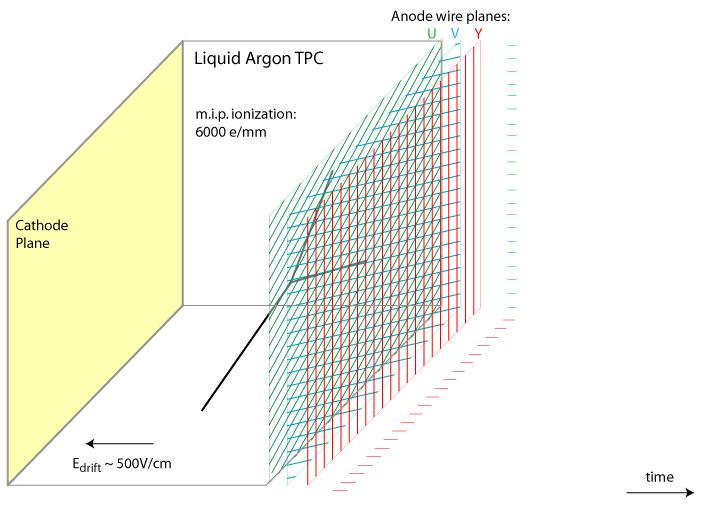
\includegraphics[width=0.9\textwidth]{signal-0.png}
	\caption{Liquid Argon TPC with wire readout: principle of operation}
	\label{fig:signal-0}
\end{figure}

The Liquid Argon Time Projection Chamber (LArTPC) is in essence a specially instrumented ionization chamber. Charges (electrons and positive ions)
created due to passage of ionizing particles through the sensitive medium (argon in this case) are subject to the effect of a uniform electrostatic
field which is created in Liquid Argon by a system of cathode and anode electrodes, which causes them to move (drift) along the field lines.
If there is an additional electrode within the Liquid Argon volume in the vicinity of the drifting charge, there will be a signal induced on it. Multiple such
electrodes (sensors) provide means for spatial characterization of the ionization charge distribution in the sensitive volume (which for example may
correspond to a particle track). Importantly, the shape of the signals on the electrode vs time is used to measure charge localization along the drift
direction (hence the term ``Time Projection Chamber''). For example, ionization electrons which are closer to the collection electrode will arrive to it sooner than
more distant ones, therefore time evolution of the signals on the affected wires will reflect distribution of the charge along the drift axis.

Current design of large scale LArTPC devices features planar arrays of wire electrodes supported by frames.
Such design contains an essential element called \textit{Anode Plane Assembly} (APA), which includes the ``collection plane'' (anode)
and two planes of sensor wires, called ``induction planes'', oriented at stereo angles with respect to each other and the collection plane.
Due to stereo angles, such arrangement allows for 2D measurement of the charge density distribution in the APA plane.
This is illustrated in Fig.~\ref{fig:signal-0}, which schematically shows the drift volume (to the left), the induction planes ``U'' and ``V'' and
the collection plane ``Y''. An important feature of such arrangement is that the \textit{same drifting charge} is measured three times as it
is detected by the three wire planes. This is further illustrated in Fig.~\ref{fig:3projections} as a schematic of drifting charge creating signals on wires,
represented conceptually as a view along the direction of the drift.

\begin{figure}[h!]
	\centering
	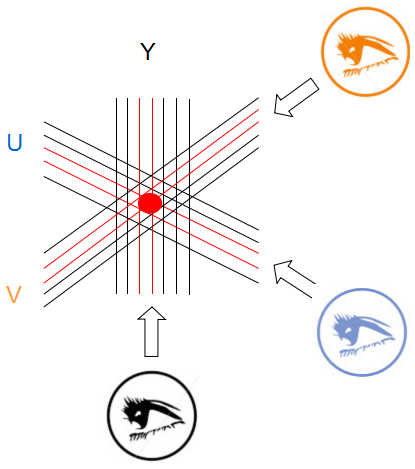
\includegraphics[width=0.65\textwidth]{uvy_2.png}
	\caption{Three projections of an object in a TPC with wire-based readout}
	\label{fig:3projections}
\end{figure}

Using just three projections to reconstruct an extended object (ionization charge density) presents challenges for event reconstruction.
Reliability and thorough characterization of the algorithms employed in this area will be critical for the systematics and other performance characteristics of DUNE.

There are a few approaches currenlty in development for event reconstruction. The ``Pandora'' toolkit, which
originated as R\&D for fine-grained calorimetry at ILC~\cite{pandora}, is being adopted to reconstruct LArTPC events.
In addition, there is a ``projection matching algorithm'' which will be used for test-beam studies with protoDUNE detector.

There is also a promising toolkit under development (called ``Wire Cell'') based on a different approach.
It performs three-dimensional imaging of events using the principles commonly applied in tomography.
As is frequently the case in tomographic reconstruction with sparse data, this may require the use memory- and CPU-intensive computing platforms.
It is likely that meeting the demands of such calculations will require adopting emerging technologies that are now becoming more common in
HEP, such as GPU or other co-processor acceleration and/or massively parallel systems such as HPC facilities.

\subsection{Pandora}
TBD


\subsection{Wire Cell}
\label{sec:wirecell}

